
\section{Problem}

FIXME: Related work and our contrasted difference.  What can we achieve that others cannot.  Why is our approach better for this particular case?  

In order to successfully control a snake robot and have it move through the environment, we need a solution for locomotion, motion planning, and handling collisions.  Since we have no exteroceptive sensors, this makes the problem challenging.  The robot is unable to sense what is right in front of it and must move blindly.  The snake could move into open space or collide with obstacles.

Part of the challenge is having no external sensors and the other part is general task-oriented control of a hyper-redundant robot.  There are many biologically-inspired locomotion strategies that live snakes in nature use to move throughout the environment.  The closest biological gait solution to moving in confined environments is the concertina gait shown in Figure \ref{bio}.

\begin{figure}
  \begin{center}
    \includegraphics[width=3in]{concertina_gait_Gans1980.jpg}
  \end{center}
  \caption{Biological Concertina Gait of a Snake in a Confined Space.  Image taken from \cite{Gans:1980p775}}
	\label{bio}
\end{figure}

This gait is characterized by a concertina motion of alternating extensions and contractions that result in a forward movement. The snake body pushes against both sides of the walls establishing anchors that allow the snake to alternate between pulling and pushing itself forward. Success of locomotion depends on the snake establishing high friction contacts with the environment with which to push and pull.

However, the differences between a real snake and our robot snake make a true implementation impossible. A real snake has the luxury of vision and olfactory sensors to provide early motion planning and a rich tactile sensing surface skin to provide feedback to its control system. Our robot snake has only the benefit of internal proprioceptive joint sensors. If we knew the exact width of the pipe walls, we could prescribe the perfect concertina motion to move through the environment smoothly.

A simple approach to making the fully anchored concertina posture, we could use the following equation:

\begin{equation}
\label{eq:naiveconc}
\alpha_i = A * \cos \left( \frac{ 2 \pi if}{N} \right)
\end{equation}

where $\alpha_i$ is the commanded joint angle for joint $i$, $f$ is the frequency or the number of sinusoidal cycles per unit segment length, $A$ is the maximum joint command amplitude, and $N$ is the number of segments on the snake.   Since there are $N$ segments, there are $N-1$ joints.  Therefore, $i \in [0,N-1)$.  This equation requires some tuning to give the right results and can result in bad postures such as that shown in Figure \ref{naiveconc}.  In order to effect locomotion, a sliding Gaussian mask should be applied to the joint command output to transition parts of the snake between fully anchored to fully straight to reproduce the biological concertina gait.

\begin{figure}
\begin{center}
\includegraphics[scale=0.5]{2_problem_1.png}
\end{center}
\caption{Improperly tuned concertina posture using equation \ref{eq:naiveconc}.}
\label{naiveconc}
\end{figure}


The difficulty of this approach is that we need a priori knowledge of the pipe width, the configuration of the snake needs to be tuned by hand for the particular snake morphology, and there is no sensory feedback to this implementation.   With no feedback, there is no adaptive behavior possible.   We need an approach that will work in environments of unknown and variable pipe width.   Our robot needs to be able to adapt its locomotion to the width of the pipe.

Our desire is to be able to prescribe any type of snake posture, for any anchor width and any snake segment length or parameters, and have the snake automaticaly assume that posture.  In order to do this, we need a means of specifying the posture and an inverse kinematics method for achieving that posture.

For both of these requirements, we use the backbone curve-fitting methodology first described by \cite{Chirikijan:1995p774}.  This method of control is to produce a parameterized curve that represents the desired posture of the snake over time. Over time the curve changes to reflect desired changes in the snake posture. Snake backbone curve fitting is achieved by finding the joint positions that best fit the snake body onto the curve. This is found either by direct calculation or a search algorithm.

An example of backbone curve fitting can be seen in Figure \ref{onePeriod}.   The parameterized curve is shown in light blue in the background.   The blue snake body in the foreground is fitted onto the curve using an iterative search algorithm for each consecutive joint. 

\begin{figure}
  \begin{center}
    \includegraphics[width=3in]{OnePeriodCurve.png}
  \end{center}
  \caption{One sine period curve}
	\label{onePeriod}
\end{figure}

A typical application would be to specify the posture of the snake using a sinusoidal curve and then applying an inverse kinematics technique to fit the snake to the curve.   The problem can be formulated iteratively as follows: for joints $i \in [0,k]$ and joint pose in space $p_i = \langle x_i,y_i,\theta_i \rangle $ are on the curve $\beta$ with parameter $t_i$, find the joint angle $a_k$ such that $p_{k+1}$ is on the curve $\beta$ and $t_k < t_{k+1}$.

For the equation $\beta$ defined as:
\begin{equation}
\label{eq:curve1}
y = A\sin(2\pi x)
\end{equation}

the equation is monotonic along the $x$ axis, so satisfying the criteria $t_i < t_{i+1}$ is the same as satisfying $x_i < x_{i+1}$.  

If the length a of snake segment is $l$, we specify a circle equation centered at the joint position $(x_i,y_i)$ with the following:

\begin{equation}
\label{eq:IKcircle}
(x-x_i)^2 + (y-y_i)^2 = l
\end{equation}

Finding solutions for the simultaneous equations \ref{eq:curve1} and \ref{eq:IKcircle} will give us possible solutions to $x_{i+1}$ and $y_{i+1}$.  For these two sets of equations, there are always at least 2 possible solutions.  We need only select the solution that satisfies the invariant condition $x_i < x_{i+1}$.   There may be more than solution.  In which case, we select the $x_{i+1}$ where $(x_{i+1}-x_i)$ is the smallest.  This prevents the snake from taking shortcuts across the curve and forces it to fit as closely as feasibly possible to the parameterized curve given the snake robot’s dimensions.

The above simultaneous equations do not have closed-form solutions and instead must be solved numerically.  This can be computationally expensive using general equation solvers.  Instead we propose a more specialized solver for this particular problem.

We choose a series of uniform samples $(q_0 ... q_k ... q_M)$ around a circle of radius $l$ centered at $(x_i,y_i)$ such that all points $q_k$ have $x_k >= x_i$.  We are looking for instance of crossover events where the line segment $(q_k,q_{k+1})$ crosses over the curve $\beta$.   Given at least one crossover event, we do a finer search between $(q_k, q_{k+1})$ to find the closest point on the circle to the curve $\beta$ and accept that as our candidate position for joint point $p_{k+1}$.   As long as we assume that the curve $\beta$ is monotonic along the x-axis and a point of the curve $\beta$ can be computed quickly given an x-value, this is a faster method of computing intersections of the circle with the backbone curve than a general numerical solver.

For instance, in Figure \ref{plot_3}, we show a curve $\beta$ described by a sine curve and a series of circles intersecting with the curve that indicate candidate locations for placing the subsequent joint on the curve.  These are used to determine the appropriate joint angles to fit the snake onto the curve.

Now that we have a means of changing the snake’s posture to any desired form given a parameterized, monotonic curve that describes the posture, we now need to form an anchoring approach that will work for arbitrary pipe widths.


\section{Anchoring}

In order to fit the anchor points to a pipe of unknown width, we need some way of sensing the walls.  Since we have no exteroceptive sensors, the best way of sensing the width of the walls is by contact.  Since we have no direct contact sensor per se, we must detect contact indirectly through the robot’s proprioceptive joint sensors.

Using the backbone curve fitting approach, we take one period of a sine curve as the template form we wish the robot to follow.  We then modify this sine period’s amplitude, at each step refitting the snake robot to the larger amplitude, until the robot make’s contact with the walls.  This establishes two points of contact with the wall which assist in immobilizing the snake body.

It is clear from Figure \ref{onePeriod} that as the amplitude of the curve increases, more segments are needed to complete the curve.  If the sine curve is rooted at the tip of the snake, this results in the curve translating towards the snake’s center of mass.  Instead, we root the sine curve on an internal segment, as seen in Figure \ref{anchor1}, so that the position of the anchor points remain relatively fixed no matter the amplitude and the number of segments required to fit the curve.

\begin{figure}
\begin{center}
\includegraphics[scale=0.5]{2_anchoring_1.png}
\end{center}
\caption{Anchor with not enough segments}
\label{anchor1}
\end{figure}

\begin{figure}
\begin{center}
\includegraphics[scale=0.4]{ref_points_pose2.png}
\end{center}
\caption{Anchor Points}
\label{fig:anchor_points}
\end{figure}


Two points of contact are not statically stable if we disregard friction.  Though friction exists in our simulation and in reality, we do not rely on it to completely immobilize our robot.  Our normal forces are often small and the dynamic and transient forces can easily cause a contact slip.  Therefore, we need at least 3 contact points to consider an anchor to be statically stable.

One way to achieve this is by adding new sine period sections to create another pair of anchors.  The amplitude of the new sine period is separate from the previous anchor’s amplitude and is represented by a new curve attached to the previous one. This way the amplitudes remain independent.  The equation to describe two sets of sine period curves with independently controlled amplitudes are as follows:

\begin{equation}
y = \mathrm{U}(x)  \mathrm{U}(2\pi-x) A_1 \sin(fx) + \mathrm{U}(x-2\pi) \mathrm{U}(4\pi-x) A_2 \sin(fx)
\end{equation}

where $f$ is the frequency and $\mathrm{U}(x)$ is a unit step function.  Or to generalize for $N$ periods and $N$ pairs of anchor points:

\begin{equation}
y = \sum_{i=0}^{N-1} \mathrm{U}(x-i 2\pi) \mathrm{U}((i+1) 2\pi-x) A_i \sin(fx)
\end{equation}


for each anchor curve amplitude $A_i$.

So now that we have the means to control the amplitude of our anchor points, we need some means of detecting that a contact is made and another to make sure the anchor is secure. 

Our approach is to gradually increase the amplitude of an anchor curve until contact with both walls has been made.  We will continue to increase the amplitude until we see significant joint error occur when fitting to the curve.  If the amplitude because larger than the width of the pipe, the snake will attempt fitting to a curve that is impossible to fit to and will experience a discrepancy in its joint positions compared to where it desires them to be.

The structure of this error will normally take the form of one or two large discrepancies surrounded by numerous small errors.  This reflects that usually one or two joints will seriously buckle against the wall, while the rest of the surrounding joints can reach their commanded position without disturbance.  An example of an anchor curve with larger amplitude than the width of the pipe is shown in Figure \ref{anchor2}.

\begin{figure}
\begin{center}
\includegraphics[scale=0.5]{2_anchoring_2.png}
\end{center}
\caption{Anchor with amplitude larger than pipe width.}
\label{anchor2}
\end{figure}

The contact is flagged once the maximum error reaches a certain threshold across all the joints of the anchor curve.  Of the joints $M$ of the anchor curve and the error $e_j$, if there exists $e_j > 0.3$ radians, than we flag a contact.  It isn’t so much that we are detecting a contact but a minimum pushing threshold against the wall.  The robot is pushing hard enough to cause joint error over an experimentally determined threshold.

If $j_k$ through $j_{k+M}$ are the joints comprising the fitted anchor curve, the error of one joint is defined by $e_k = |\phi_k-\alpha_k|$.  The maximum error is defined by $e_{max} = \mathrm{max}(e_k, e_{k+1} \cdots e_{k+M-1}, e_{k+M})$.

The amplitude is initially changed by large increments to quickly find the walls.  Once the threshold has been reached, the current and last amplitude are marked as the max and min amplitudes respectively.  We then proceed to perform a finer and finer search on the amplitudes between the max and min boundaries until we reach a snug fit that is just over the error threshold.  This is a kind of numerical search(?).

The pseudocode for this algorithm is as follows:


\begin{algorithm}
\caption{Anchor Fitting}          % give the algorithm a caption
\label{alg:anchor}
\begin{algorithmic}

\State $\hat{A} \Leftarrow 0$
\State $A_{min} \Leftarrow 0$
\State $A_{max} \Leftarrow \infty$
\State $\delta A \Leftarrow 0.04$

\While{$ (A_{max}-A_{min} >= 0.001) \And (\delta A >= 0.01)  $} 

  \State $\hat{A} \Leftarrow \hat{A} + \delta A$
  \State $e_{flag} \Leftarrow \mathrm{setAnchorAmp}(\hat{A})$
 
  \If { $\neg e_{flag}$ }
    \State $A_{min} \Leftarrow \hat{A}$
  \Else
    \State $A_{max} \Leftarrow \hat{A}$
    \State $\delta A \Leftarrow \delta A / 2$
    \State $\hat{A} \Leftarrow A_{min}$
    \State $\mathrm{setAnchorAmp}(\hat{A})$

  \EndIf

\EndWhile

\end{algorithmic}
\end{algorithm}

The main objective of this code is to reduce the difference between maxAmp and minAmp as much as possible.  minAmp and maxAmp are the closest amplitudes under and over the error threshold respectively.  The function setAnchorAmp() sets the amplitude, performs the curve fitting, and reports back any error condition as described earlier.  Once this algorithm is complete, we have made a successful anchor with two contact points under compression without the fitted anchor curve being distorted by joint buckling.

\section{Curves}

When we describe curves for use in backbone curve fitting, they must be assigned to a frame of reference and usually have a starting point.  Most often, the frame of reference chosen is one of the local segment frames on the snake body.  However, sometimes we could choose the global frame if we wanted to navigate or probe something specific in the environment.  The local frame curves that we use all start from a specific body segment and sprout from that segment like a plant.  We say that this curve is rooted in segment X. 


\section{Behaviors}

Our method of control is a behavior-based architecture that is charged with reading and tasking the servo-based motor controllers of each joint.  Each behavior may be a primitive low-level behavior or a high-level composite behavior composed of multiple sub-behaviors.  Furthermore, a behavior may have complete control of every joint on the snake or the joints may be divided between different but mutually supporting behaviors.  This architecture allows us to achieve a hierarchy of behavior design as well a separation of responsibilities in task achievement.  For instance, the back half of the robot could be responsible for anchoring, while the front half could be responsible for probing the environment as seen in the example architecture in Figure \ref{behaviors1}.

\begin{figure}
\begin{center}
\includegraphics[scale=0.5]{2_behaviors_1.png}
\end{center}
\caption{Separation of functionality.}
\label{behaviors1}
\end{figure}

Each behavior in the behavior-based architecture is time-driven.  It is called periodically by a timer interrupt to compute the next commands for the following time-step.  This could be variable time or constant time, but to make our behavior design simple, we use 10ms constant time steps in our simulation.

At each time step, the state of the robot is captured and driven to the behaviors.  The data includes a vector of joint angles $\phi_i$, a vector of commanded angles $\alpha_i$, and a vector of maximum torques $m_i$.  These values were described in the previous section X.  The output of each behavior is a vector of new commanded angles $\hat{\alpha}_i$, a vector of new max torques $\hat{m}_i$, and a vector of control bits $c_i$.  The values of $\hat{\alpha}_i$ can be any radian value within the joint range of motion or it can be NULL.  Likewise, the new max torque of $\hat{m}_i$ can be any non-negative max torque threshold or NULL.  The NULL outputs indicate that this behavior is not changing the value and if it should reach the servo-controller, it should persist with the previous value.

The bits of the control vector, $c_i$ , are either 1, to indicate that the behavior is modifying joint i, or 0, to indicate that it has been untouched by the behavior since its initial position when the behavior was instantiated.  This control vector is to signal the activity to parent behavior that this part of the snake is being moved or controlled.  The parent behavior does not need to respect these signals, but they are needed for some cases.

Our behavior-based control architecture follows the rules of control subsumption.  That is, parent behaviors may override the outputs of child behaviors.  Since we can also run multiple behaviors in parallel on different parts of the snake, sometimes these behaviors will try to control the same joints.  When this happens, the parent behavior is responsible for either prioritizing the child behaviors or adding their own behavior merging approach.

Asymmetric behaviors that run on only one side of the snake such as the front are reversible by nature.  That is, their direction can be reversed and run on the back instead.  All behaviors with directional or asymmetric properties have this capability..

Finally, parent behaviors can instantiate and destroy child behaviors at will to fulfill their own control objective.  All behaviors are the child of some other behavior except the very top root-level behavior which is the main control program loaded into the robot and responsible for controlling every joint.  The root behavior is responsible for instantiating and destroying assemblages of behaviors to achieve tasks as specified in its programming.  We will discuss some of these behaviors and child behaviors in the following sections.

\section{Smooth Motion}
\label{sec:smooth}

We desire the motion of our snake robot to be slow and smooth in nature.  It does us no benefit for the motion to be sudden and jerky.  Moments of high acceleration can have unintended consequences that result in our anchor points slipping.  Either collisions with the environment or transient internal dynamics can cause the anchor points to slip.

Our method of ensuring smooth motion is to take the initial and target posture of the joints of the snake, perform linear interpolation between the two poses, and incrementally change the joint angles along this linear path.  For instance, if the initial joint angles are ${s_0 ... s_n}$ and the target joint angles are ${t_0 ... t_n}$, the interpolated path for each joint $j$ is found by $g_{jr} = s_j + (t_j – s_j) * (r/100)$ for $r \to {0, 100}$, for 100 interpolated points on the linear path.  The resultant motion is a smooth transition from initial to target posture as seen in Figure \ref{smooth1}.

\begin{figure}
\begin{center}
\includegraphics[scale=0.5]{2_smooth_1.png}
\end{center}
\caption{Smooth motion from interpolation of posture.}
\label{smooth1}
\end{figure}

This is the definition of the HoldTransition behavior.  When it is instantiated, it is given an initial pose vector $S$ and target pose $T$, where some values of $t_i$ in $T$ and $s_i$ in $S$ may have NULL for no command.   At each step of the behavior, using the equation $g_{jr} = s_j + (t_j – s_j) * (r/100)$, $r$ is incremented to compute the new joint command.  If $t_j$ is NULL, then $g_{jr} = s_j$.  Once $r = 100$, it returns True on step() and on all subsequent steps, $g_j = t_j$.


\section{Behavior Merging}

\label{sec:merge}

There are a few methods for merging behaviors that overlap in some way.  One way of the previous section is for two behaviors to overlap temporally and using the HoldTransition behavior to handle a smooth transition from one configuration to another.

In the event that two behaviors control adjacent sets of joints or overlap their control in some way, a conflict resolution is method is needed to not only select the proper command for contested joints, but to prevent either behavior from negatively affecting functionality of the other by modifying any positional assumptions or introducing any unintended forces or torques to the other side.

A common occurrence is that two behaviors may try to control the same set of joints at the same time or otherwise.  This is a conflict that requires resolution by the parent behavior.  In this section we present three different ways to merge the outputs of different behaviors as means of conflict resolution.  They are, in the order presented, the precedence merge, the splice merge, the convergence merge, and the compliance merge respectively.

Given that all child behaviors have an ordering, the default resolution method is to take the first behavior’s control output over all others.  This is called precedence merging.  An ordering is always specified by the parent at the time it instantiates the child behaviors.  If the first behavior’s output is NULL, then it goes to the next behavior and so on until a non-NULL value is found or the last behavior returns a NULL, in which case the parent also returns a NULL unless the parent otherwise specifies.

Precedence merging can be crude when trying to maintain a stable and immobilized position in the environment.  Sudden changes at the behavior-boundary can cause jarring discontinuities on the snake’s posture and result in loss of anchoring as seen in Figure \ref{merging1}.  A more finessed approach would disallow these discontinuities and provide a non-disruptive merging.  The first approach that does this is the splice merge.

\begin{figure}
\begin{center}
\includegraphics[scale=0.5]{2_merging_1.png}
\end{center}
\caption{Discontinuity in behaviors results in clash of functionality.}
\label{merging1}
\end{figure}

In the event that two behaviors overlap, we have the option of having a hard boundary between the behaviors centered on a single joint. Except in the rare case that both behaviors want to command the splice joint to the same angle, it is highly likely that the merge will be discontinuous.  In order to ensure that positional assumption is maintained for both behaviors, the behaviors must be spliced so that neither behavior disrupts the other.

If the splice joint is $j_s$, behavior A controls joints $j_0$ through $j_s$, behavior B controls joints $j_s$ through $j_{N-1}$, $S_{s-1}$ is the body segment connected to $j_s$ in behavior A, and $S_s$ is the body segment connected to $j_s$ in behavior B, we have the situation shown in Figure \ref{merging2}a.  If behavior A commands $j_s$ to $\alpha_a$ to put segment $S_s$ in the position shown in Figure \ref{merging2}b and conversely, if behavior B commands $j_s$ to $\alpha_b$ to put segment $S_{s-1}$ in the position shown in Figure \ref{merging2}c, the two behaviors can be spliced discontinuously with no disruption to either behavior by setting $j_s$ to $\alpha_s = \alpha_a + \alpha_b$.  The result is shown in Figure \ref{merging2}d.

\begin{figure}
\begin{center}
\includegraphics[scale=0.5]{2_behaviors_2.png}
\end{center}
\caption{Splice joint and connecting segments.}
\label{merging2}
\end{figure}

This is the behavior splicing approach because it stitches the behaviors together in a clinical way to ensure proper functionality of both.  Its primary role is to connect behaviors with discontinuous conflicts on the behavior boundary and whose positions must be maintained for functional purposes.  For more fuzzy continuous boundaries, we use the convergence merging approach.

For the two behaviors shown in Figure \ref{merging3}a and \ref{merging3}b, the resultant convergence merge is shown in Figure \ref{merging3}c.  For this approach, there is no discrete boundary but one behavior converging to another over several joints.  For a given joint $j_i$ somewhere in this convergence zone, and the commanded values for behaviors A and B being $\alpha_a$ and $\alpha_b$, the converged command value for $j_i$ is computed by:

\begin{equation}
\label{equ:slide}
\alpha_i = \alpha_a + (\alpha_b – \alpha_a) / ( 1 + \exp(i-c))
\end{equation}

where $c$ is a calibration parameter that controls the magnitude and location of the convergence along the snake.  As $c \to +\infty$, $\alpha_i \to \alpha_b$.  As $c \to -\infty$, $\alpha_i \to \alpha_a$.  In practice, $|c| < 20$ is more than sufficient for complete convergence to one behavior or the other.  The $i$ parameter in the exponent ensures that the convergence value is different for each of the neighboring joints.  This produces the effect shown in Figure \ref{merging3}c.

\begin{figure}
\begin{center}
\includegraphics[scale=0.5]{2_behaviors_3.png}
\end{center}
\caption{Convergence merge.}
\label{merging3}
\end{figure}

If we modify $c$, this gives us a control knob on the merge and can be moved up and down.  If we move $c \to +\infty$, behavior B takes complete control of the snake.  If we move $c \to -\infty$, behavior A takes control of the snake.  $c$ can be changed over time to create a sliding transition effect with a convergence boundary.  In fact, this is the basis for a behavior called HoldSlideTransition.

A fourth and final way for two behaviors to be merged is the compliance merge.  This is the case where two behaviors are not adjacent but are far away from each other, but still interfere with each other somehow by inflicting unwanted forces and torques between the behaviors.

A compliance merge resolves this by selecting a group of joints between the two behavior’s joint sets to be compliant or non-actuated.  This has the result of absorbing any forces or torques transmitted by either behaviors and mechanically isolating one side of the snake from the other.  An example is shown in Figure \ref{merging4}.

\begin{figure}
\begin{center}
\includegraphics[scale=0.5]{2_behaviors_4.png}
\end{center}
\caption{Compliance merge.}
\label{merging4}
\end{figure}

\section{Compliant Motion}

In the previous section, we mentioned compliance but not our implementation.  Compliant motion is a much used technique in robotics and has been discussed widely (cite).  The two approaches are either passive or active compliance.  Our approach is to use passive compliance since we have no means to detect contact or sense obstacles.

Passive compliance is achieved by changing the settings on the max torque parameter of each joint’s servo controller.  We use a high setting for active motion, a low setting for compliant motion, and zero for keeping the joint unactuated.

Besides using a compliance merge to mechanically isolate two behaviors, we also use compliance as an exploration strategy.  Since we have no exteroception, the only way to discover walls and obstacles is to collide with them.  Compliant impacts with obstacles have a couple benefits.  It prevents the force of the impact from transmitting to the body of the snake and possibly causing anchor slip.   It also allows the joints of the snake to give out and take the shape of the environment around it.  

This latter benefit is one of our primary means of sensing and exploring the environment.  By passively letting the snake robot assume the shape of the environment, it guides our mapping and our locomotion.  Until we have mapped out open space and boundaries, we have no way of directing our robot towards them beyond colliding with the unknown.

\section{Stability Assurance}

\label{sec:stability}

In a previous section on smooth motion, we discussed an interpolation technique to smoothly transition from one posture to another.  The primary motive of this was to keep the parts of the snake body that are immobilized from being destabilized by transient forces and causing anchor slip.  Static forces from prolonged pushing against an obstacle or wall are a separate matter.

For a pose transition that has a sufficiently large number of interpolation steps of sufficiently large duration, we can reasonably be assured that no transient forces from dynamics or collision will cause anchor slip because we are moving very very slowly.  However, sufficiently long transition times for reliability may be impractical for applications, since times for a simple transition can be upwards of 1-2 minutes using a conservative approach.  For a robot that performs hundreds of moves that require transitions, this is an unacceptable approach.

If we focus on being able to detect transient forces on the snake body instead, we can use this to control the speed of our movements instead of a one-size-fits-all approach of long transition times for all motion.  We have developed a heuristic technique to do just this.

Our approach is to use our only source of information, joint angle sensors, as make-shift stability monitors of the entire snake.  That is, if all the joints stop changing within a degree of variance, we can call the whole snake stable.  Once we have established that the snake is stable, we can perform another step of motion. 

For each, we compute a sliding window that computes the mean and variance of the set of values contained in.  If at every constant time step, we sample the value of some joint $i$ to be $\phi_{it}$, then we compute:

\begin{equation}
\mu = \sum_{t = j-K}^{j} \frac{\phi_{it}}{K}
\end{equation}
\begin{equation}
\sigma^2 = \sum_{t=j-K}^{j} \frac{(\phi_{it} – \mu)^2}{K}
\end{equation}

$K$ is the width of the sliding window or the sample size used for computing the variance.  This and the time step size $\delta t$, are used to determine the resolution and length of variance computation.  In our implementation, with some exceptions, we use $\delta t = 1\mathrm{ms}$ and $K = 20$.  That is, for $N$ joints, we compute the variance of each joint’s angle for the last 20 readings once every 1ms.  This may be changed and retuned depending on the available computing resources, the resolution of the sensors, and the sensor’s sample rate.

Finally, we can determine if the snake is stable if all of the joint variances fall below a threshold $S_v$ and stay that way for over time $S_t$.  In our case, we set $S_v = 0.001$ and $S_t = 50\mathrm{ms}$.

We are primarily interested in preventing anchor slip.  Most often, it is not necessary to wait for the entire snake to hold still before moving.  Instead, we can focus just on the joints in the neighborhood of the anchor points.  By computing just the variances of the joints in the local neighborhood of the anchor points, we can determine local stability.  Using local stability, we gain some confidence that our anchor points do not slip between motion steps.

In order to use this concept of local stability, we need to have some indication of which joints to monitor and which to ignore.  Fortunately, the control vector c, output of the behaviors mentioned in a previous section, is just the kind of information we need to know where to direct our local stability attention.  If the values of a control vector indicate ‘0’, this means that these joints are not modified by the behavior and should remain stable before performing another move step.  If the values are ‘1’, these joints are actively modified by the behavior and we should not expect these joints to remain stable between move steps.  The behavior prescriptively tells us how it should behave and the stability system processes it to accommodate.

\section{Adaptive Step}

%Show the behavior sequence in high-level terms.  Show graphics.

%Explain each behavior step in terms of the concepts we already learned.

Using these tools at our disposable, we can now build a suitable locomotion behavior for an unknown pipe with no exteroception.  The entirety of our designed behavior is shown in Figure \ref{adaptive_step} and is called the adaptive concertina gait, a biologically-inspired gait based on the concertina gait but modified for the change in sensors.  The behavior is divided into 6 states, and each level of Figure \ref{adaptive_step} shows one of those states.  We describe the states as follows:


\begin{figure}
\begin{center}
\includegraphics[scale=0.8]{AdaptiveStep.png}
\end{center}
\caption{Adaptive Step Concertina Gait}
\label{adaptive_step}
\end{figure}

1) Rest-State (Initial): Rest-State is the initial fully anchored posture of the snake robot.  This is our initial pose and it acts as a stable platform from which exploratory or probing behaviors can be executed to sense the environment with little chance of slips or vibration due to the multiple anchor contact points.  There is no other action here than to hold the posture that it was already in.  The Rest-State is the initial state and the final state of the concertina gait.

2) Front-Extend:  In the Front-Extend state, the forward segments are gradually transitioned from their initial position to a straight-forward position.  The joints are compliant to the boundaries of the environment to accommodate turns in the pipe.

3) Front-Anchor:  The Front-Anchor state takes the extended portion of the snake and attempts to establish an anchor to the pipe as far forward as possible.  The locomotion distance is maximized the further forward the front anchor is.

4) Back-Extend:  The Back-Extend state follows a successful Front-Anchor event.  All anchors established in the back segments are gradually extended until they are straight.  Again, the joints are compliant so that they can conform to the walls of the environment.

5) Back-Anchor:  The Back-Anchor state involves establishing multiple anchors with the remainder of the body segments.

6) Rest-State (Final):  Upon conclusion of the Back-Anchor state, a single step of the adaptive concertina gait is complete and the snake is now in the Rest-State.  From here we can do probing of the environment or perform another step forward.

A successful transition through all the states results in a single step.  Multiple steps are used to travel through the environment.  We describe no steering mechanism for this locomotion gait because the robot has no means to sense the environment in front of it.  However, the robot’s compliant posture will adapt to any junctions or pipe curvature and follow it.

We now describe the implementation of each of these states and their composition of behaviors.



\subsection{Front-Extend}

%GRAPHIC
%Merge(
%FrontExtend ← HoldSlideTransition ← Transition,
%HoldPosition
%)
\begin{figure}
\begin{center}
\includegraphics[scale=0.5]{2_adaptive_1.png}
\end{center}
\caption{Front-Extend behavior assembly.}
\label{adaptive1}
\end{figure}

%Convergence merge of 0.0 extension and anchored state.  Precedence merge of FrontExetend and HoldPosition.  HoldPosition holds back half while FrontExtend controls front.  Passes extended state to HoldSlideTransition.  This manages convergence merge and slide with a Transition behavior to handle each step. 

From the fully anchored Rest-State stage, the goal of the Front-Extend stage is to release the front anchors and stretch the front half of the snake as far forward as possible without compromising the rear anchors.  The further forward we can extend, the further the snake can travel in a single step.

If the extended snake arm makes a lateral impact, the walls will guide the movement of the snake but not otherwise hinder the behavior.  In the event of an actual obstruction, the tip’s movement will stop.  We are able to track whether the position of the tip hasn’t moved overtime and are able to set a flag to abort the behavior at the current posture.

Its implementation consists of 4 behaviors arranged as shown in Figure \ref{adaptive1}.  We explain each behavior's functionality.

\textbf{HoldPosition:} The purpose of this behavior is to output the same joint commands indefinitely.  It is instantiated with a vector of joint commands, and it continues to output these joint commands until termination.  In this case, it is instantiated with the entire initial anchored posture of the snake from Rest-State and continues to output this posture.  The behavior’s output is gradually subsumed by the growth of the FrontExtend behavior in a precedence merge.  HoldPosition is placed 2nd in the behavior ordering at the root level for this reason.

\textbf{Transition:} This behavior’s purpose is to take an initial and final pose and interpolate a transition between the two, outputting the intermediate postures incrementally.  The number of interpolated steps used to transition between the poses is set by the parent behavior.  It is often a function of how much difference there is in the initial and final poses.  The clock-rate is dependent on the parent behaviors. Once it reaches the final pose, it returns a flag and continues to output the goal pose indefinitely until reset or deleted.  Here it is instantiated by the HoldSlideTransition behavior and reset each time it needs to make a new move command.

\textbf{HoldSlideTransition:} This behavior was first mentioned in section \ref{sec:merge} and implements the equation \ref{equ:slide}.  Its role is to use a convergence merge to transition from one posture to another.  The convergence parameter $c$ is incremented over time to slide the convergence from the front to the back of the snake, to smoothly transition from the fully-anchored posture to the back-anchored and front-extended posture.

For each change in $c$, the Transition behavior is set up to interpolate smooth motion between the two postures.  Once the Transition behavior completes, $c$ is incremented and Transition is reset to the new initial and final postures.  $c$ is changed from 8 to 20 while using the joint numbers as the indices in the convergence merge equation shown in X, assuming that the joint numbering starts at 0 at the front tip.  An example of the HoldSlideTransition behavior in action is shown in Figure \ref{merging3}.

\textbf{FrontExtend:}  Finally, the FrontExtend behavior creates HoldSlideTransition as a child behavior and gives it its initial and final posture.  It passes through the output of HoldSlideTransition.  It also monitors the pose of the snake tip to see if any obstructions are encountered.  If the pose remains stationary for a period of time, an obstruction is declared and the behavior is halted.  The behavior returns a collision flag.

\subsection{Front-Anchor}

\begin{figure}
\begin{center}
\includegraphics[scale=0.5]{2_adaptive_2.png}
\end{center}
\caption{Front-Anchor behavior assembly.}
\label{adaptive2}
\end{figure}

%GRAPHIC
%Merge(
%FrontAnchor -> FrontAnchorFit, 
%    |
%   V
%HoldTransition
%)

Once the front-half of the snake has been extended by the Front-Extend stage, the next step is to place the first anchor using the already extended segments.  The complete posture of the snake is submitted to a HoldTransition behavior while the front half of the posture is modified by the FrontAnchorFit behavior.

This stage attempts to create a 3-point anchor that is created with the previously extended segments.  The anchor is rooted at an internal joint starting from the merge joint 7 giving 8 segments with which to create the anchor.  In the event that not enough segments are available to create the full anchor, the anchoring process is restarted with +2 more segments by moving the root inward by 2 joints.  

On successful completion of the 3-point anchor with the available segments, a test is performed to see if the anchor is secure, called a jerk-test.  This is accomplished by a sudden rotation of four joints adjacent to the merge joint not on the side of the front anchor.  While tracking the position of the anchor segments, if the anchored portion of the snake moves appreciably from the jerk-test, the anchor is deemed insecure, and the anchoring process is restarted with 2 more segments.

Whenever the merge joint is moved inwards, this also results in the contact positions of the anchor points moving inward as well.  This can be useful for changing the anchor locations if no stable purchase is found, but also reduces the step distance of the gait by reducing the extension length.

The composition of the behaviors is shown in Figure \ref{adaptive2} and described as follows:

\textbf{HoldTransition:}
This behavior is originally initialized with the complete posture of the snake at the outcome of the Front-Extend stage.  The front portion is laterally modified by the FrontAnchor behavior whenever new changes are required to the front anchor shape.  The behavior is stepped and drives the robot joints for smooth transitions.

Though the FrontAnchor behavior has priority over the HoldTransition behavior, FrontAnchor almost never drives an output but instead laterally modifies the HoldTransition behavior.  Therefore, the HoldTransition behavior is the primary driver of the snake robot.

\textbf{FrontAnchor:}
This behavior has complete responsibility for the entire anchoring and testing process.  It creates a 3-point anchor for static stability instead of the 2-point anchors previously described in section 2.1.  This is because this will be the only anchor to the environment in the next stage.  Complete secureness is required to avoid any slip conditions.

A 3-point anchor is created with a cosine curve of period 2.5pi shown in Figure \ref{frontanchor1}.  The FrontAnchor behavior gradually increases the amplitude of this curve.  As the amplitude increases, more and more segments are required to complete the fit.  Should the curve be longer than the available number of segments, the anchoring process is restarted with the merge joint moved back 2 joints.

The anchoring process is halted after search algorithm 2 completes.  The behavior then performs a jerk-test to determine if the anchor points are secure.  If k’th joint is the merge joint, then the joints [k+1,k+4] are rapidly changed in the following sequence:  [(0,0,0,0), (-60,-60,-60,-60), (0,0,0,0), (60,60,60,60)].  These joints are directly controlled by the FrontAnchor behavior to create sudden motion and override the parallel HoldTransition behavior that normally performs smooth motion.

A secure anchor will register little movement in the anchor segments while an insecure anchor will move a great deal.  This movement is tracked through kinematics and assumes that the back anchors are secure and stable.  Once the deviation in position of the anchor segments is below a certain threshold, than we determine that this is a secure anchor and return success.

\textbf{FrontAnchorFit:} 
This behavior is responsible for computing the curve-fitting process described at the beginning of section 2.  It determines the correct joint orientations for a given curve.  The curve is input by the FrontAnchor behavior and modified accordingly.  The FrontAnchorFit behavior performs an efficient curve-fitting process assuming the curve starts rooted at the merge joint on the behavior boundary shown in Figure \ref{frontanchor1}.

\begin{figure}
\begin{center}
\includegraphics[scale=0.5]{2_frontanchor_1.png}
\end{center}
\caption{Posture that creates a 3-point anchor.}
\label{frontanchor1}
\end{figure}


\subsection{Back-Extend}

\begin{figure}
\begin{center}
\includegraphics[scale=0.5]{2_adaptive_3.png}
\end{center}
\caption{Back-Extend behavior assembly.}
\label{adaptive3}
\end{figure}

%GRAPHIC
%Merge(
%BackExtend
%    |
%    V
%HoldTransition
%)

After the front anchor has been securely established, the next stage’s role is to remove the back anchors and extend the back half of the body straight.  If the environment prevents the back half from being straight, the joints are compliant to the environment and will extend as far as they are allowed.

The behaviors are shown in Figure \ref{adaptive3} and described as follows:

\textbf{BackExtend:}
This behavior simply takes all the joints on one side of the merge joint behavior boundary and commands their values to be 0.0.  It also sets all of these joints to have low torque to ensure compliant motion.  These values are sent laterally to the HoldTransition behavior.

\textbf{HoldTransition:} 
This behavior is initialized to the posture from the outcome of the Front-Anchor stage.  It receives as input from the FrontExtend behavior, the new straight 0.0 joint positions.  It manages the smooth motion from the back anchored position to the back extended position.


\subsection{Back-Anchor}

\begin{figure}
\begin{center}
\includegraphics[scale=0.5]{2_adaptive_4.png}
\end{center}
\caption{Back-Anchor behavior assembly.}
\label{adaptive4}
\end{figure}

%GRAPHIC
%Merge(
%BackAnchor -> FastLocalCurveFit, 
%    |
%    V
%HoldTransition
%)

The purpose of this stage is form the 2-point anchors described in section 2.1 with the remaining extended segments of the back half of the snake.  The sine curves are joined together with the front anchor cosine curve to make a continuous splice merge and produce a complete anchored posture of the whole snake.

New pairs of anchor points are created, using one period of a sine curve each, until all of the remaining back segments are used up.  At each anchor pair, we use the adaptive anchoring algorithm 2 to detect contacts.  However, we do not perform a jerk-test like in the Front-Anchor stage because we only have the front anchor as our reference point and no extra joints to perform the jerking motion.  Furthermore, it is not as critical to determine if the back anchors are secure since there are more of them, and we have confidence in the security of our front anchor.


The behaviors are shown in Figure \ref{adaptive4} and described as follows:

\textbf{HoldTransition:} 
This behavior fulfills the same role as all of the other instances.  It takes the initial posture at the outcome of the previous stage and maintains that posture until modified by the primary behavior, BackAnchor.   It manages the smooth transition between postures.

\textbf{BackAnchor:} 
This behavior performs the anchor contact algorithm 2, modifies the curve parameters, and continues to add anchor pairs until it runs out of segments.  It creates the FastLocalCurveFit behavior as a child behavior.

\textbf{FastLocalCurveFit:} 
This behavior parameterizes the curves representing the series of back anchor curves of varying amplitudes.  It is also responsible for efficiently computing the joint positions to fit the snake to the curves.  Furthermore, it accepts compliance in the curve-fitting process between each anchor pair.  That is, at each merge joint between two anchor pairs, compliance is to find the best anchor posture and the posture is saved for the remainder of the stage.


\section{Analysis}


Our theoretical contribution is a quantitative analysis of the trade-space between environmental characteristics, snake robot morphology, and locomotion control parameters.  That is, given a snake robot morphology and control parameters, what types of environments can we successfully explore.  Conversely, given a specific environment, what robot morphology and control parameters are required to successfully explore it.

First we will perform an analysis of the trade-space for forming a 3-point stable anchor in a smooth pipe.  A 3-point anchor is shown in Figure \ref{param_1} and is the minimum number of contact points required to form a stable anchor.  This posture will hold the body of the snake rigid and prevent it from translating or rotating within a threshold of external force and torque.

We will define and quantify the parameters that describe this system: the environment, the robot, and the control.

Our particular environment of a smooth pipe can easily be described with one parameter, the pipe width $W$.

The complete snake robot morphology can be described by 3 parameters: segment width $w$, segment length $l$, and number of segments $n$.

Finally, control of the robot is achieved by fitting the body of the snake onto a curve described by a sinusoid.  The parameters for control are the values of amplitude $A$ and period $P$, where $y = A \cos(\frac{2 \pi x}{P})$.  

\begin{figure}[htb]
\begin{center}
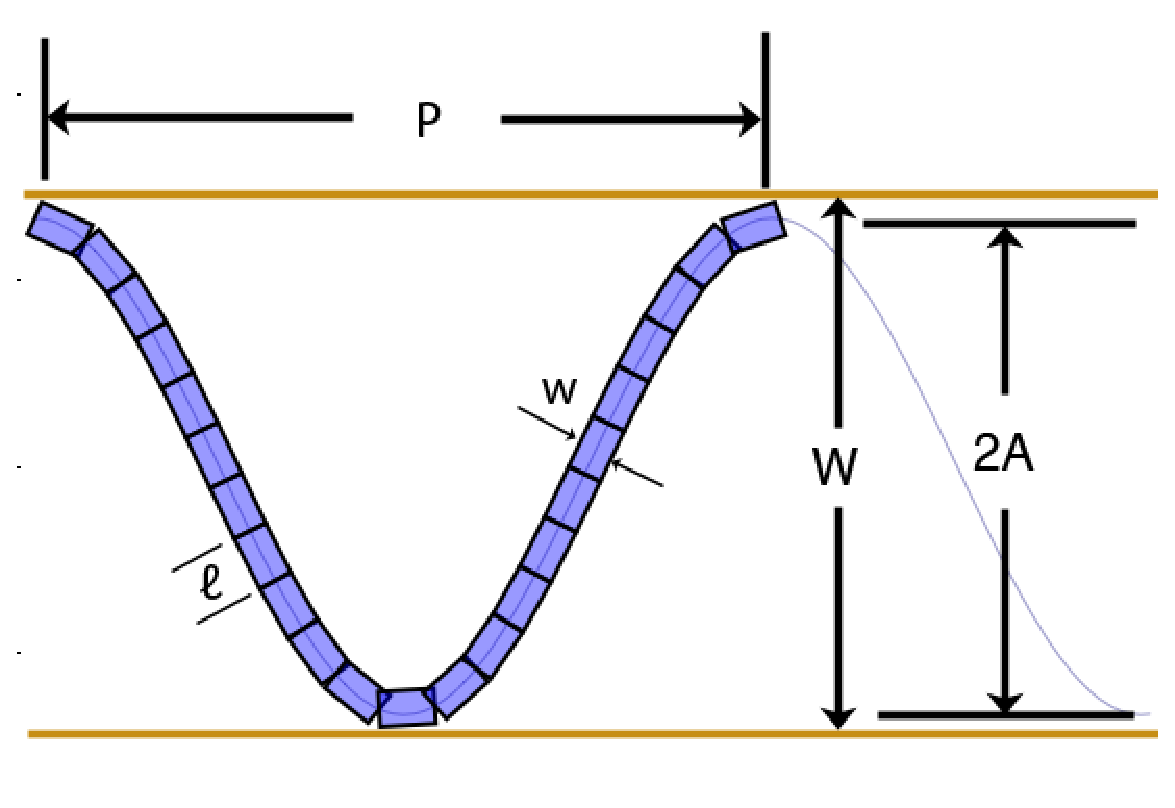
\includegraphics[scale=0.5]{CurveDiagram}
%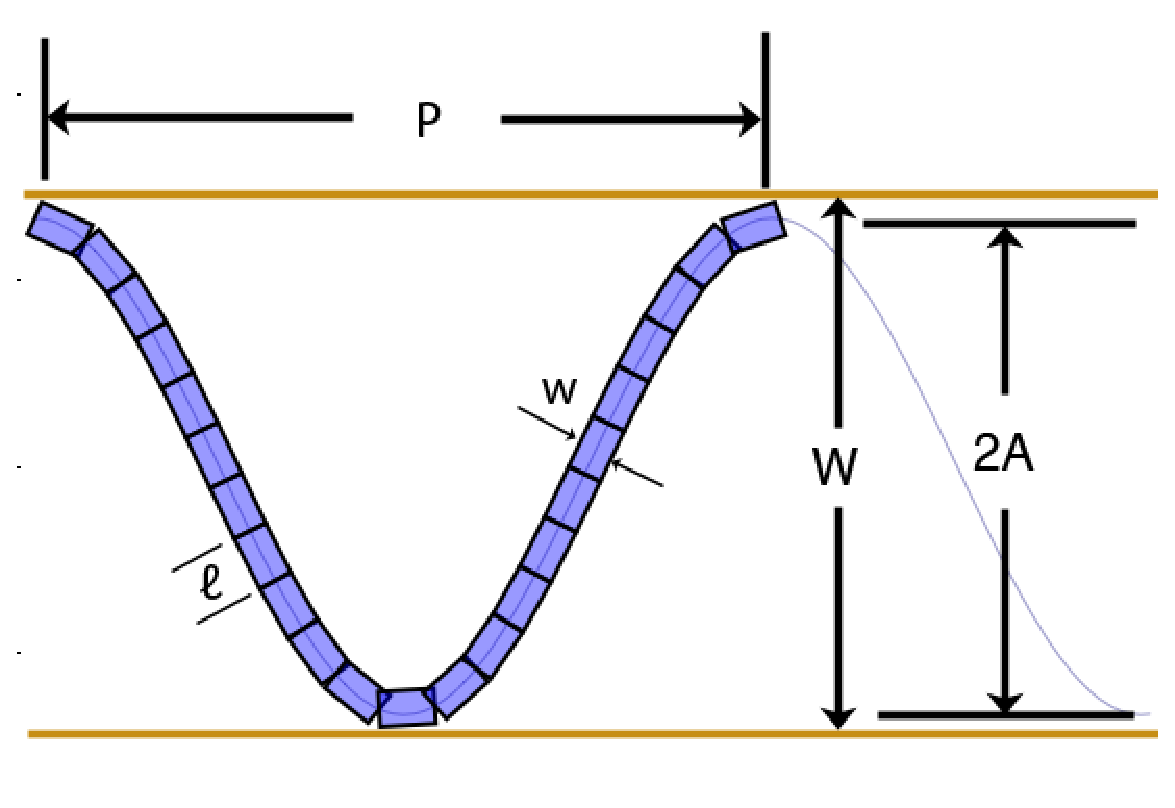
\includegraphics{CurveDiagram}
\end{center}
\caption{Parameterization of 3-point stable anchor in a smooth pipe.}
\label{param_1}
\end{figure}

\subsection{Case: Snake as a Curve}

We first consider the degenerate case where $l = 0$, $w = 0$, and $n = \infty $.  This results in a snake that has no width and an infinite number of joints.  Essentially, the snake body equals the curve equation.  Since $w = 0$, this results in $ 2A = W $.  This is shown Figure \ref{deg_1}.

\begin{figure}[htb]
\begin{center}
\includegraphics[scale=0.5]{DegenerateCurve}
%\includegraphics{DegenerateCurve}
\end{center}
\caption{3-point stable anchor with $w = 0$, $l = 0$, and $n = \infty $.}
\label{deg_1}
\end{figure}

We define $L$ to be the total length of the snake which can be computed from the equation of the curve.

\begin{equation}
f(x) =  \frac{W}{2} \cos \left( \frac{2 \pi x}{P} \right) 
\end{equation}

Equation 1 is the equation of the curve with $P$ the period, $W$ the width of the pipe.   We can plug $f(x)$ into the equation for computing arc length shown in Equation 2 and 3:

\begin{equation}
L = \int_{0}^{P} \sqrt{f'(x)^2 + 1} \,\,\, dx
\end{equation}

\begin{equation}
L = \int_{0}^{P} \sqrt{\left( \frac{-W \pi}{P} \sin \left( \frac{2 \pi x}{P} \right)  \right)^2 + 1} \,\,\, dx
\end{equation}

This integration can not be solved analytical and must be solved by plugging in values for $P$ and $W$ and computing $L$ numerically.  In our control methodolgy, $P$ is usually held fixed and the width of the environment is always changing, so $W$ is always varying.  Here we show a plot holding $P$ fixed for various values while changing the value of $W$ in Figure \ref{plot_1}.

\begin{figure}[htb]
\begin{center}
\includegraphics[scale=0.6]{2011_01_23_Plot_DegenerateAnchor}
\end{center}
\caption{Plot of snake arc length $L$ for various values of $W$ and $P$.}
\label{plot_1}
\end{figure}

This plot shows that when pipe width $W \to \infty$, the length $L$ converges to a constant slope of $\frac{dL}{dW} = 2$ and $L = 2W \,, \forall P$ as $W \to \infty$.  This can be seen by approximating the 3-point anchor and cosine curve as a triangle with a base of $P$ and a height of $W$, and the vertices on the anchor points.  Increasing $W$ will achieve the above results.

The difference in $L$ becomes large for different values of $P$ when $W$ is small.  Once $W$ becomes sufficiently large, $W$ dominates and the period becomes less of a factor.   Given that our application involves tight quarters, we are likely to find typical values of $W$ to be small and $P$ will vary depending on the context.

\subsection{Case: Snake with Width}

We now consider the case where $l = 0$, $n = \infty$, but $w > 0$.   This in effect creates a continuous snake robot with infinite joints but has a thickness to it.  To determine the total length of the snake given a pipe width $W$, a control period $P$, and a segment width of $w$, we first determine the equation of the curve:

\begin{equation}
f(x) =  \frac{W-w}{2} \cos \left( \frac{2 \pi x}{P} \right) 
\end{equation}

Since the snake centers its body on the curve, it has space of $\frac{w}{2}$ on either side of it.  We start the cosine amplitude at $\frac{W}{2}$ and substract $\frac{w}{2}$ as the width of the snake increases.  This results in equation 4.

If we plug the $f(x)$ into the arc length equation, we get the snake length for given $W$, $P$, and $w$:

\begin{equation}
L = \int_{0}^{P} \sqrt{\left( \frac{-(W-w) \pi}{P} \sin \left( \frac{2 \pi x}{P} \right)  \right)^2 + 1} \,\,\, dx
\end{equation}

Holding $P = 1$, and increasing the pipe width $W$ for different values of $w$, we get the following plot shown in Figure \ref{plot_2}.  This plot captures the intuition that a snake robot is not able to explore a pipe that is thinner than the robot's body width.  However, once you enter a pipe where $W > w$, the plot takes on the same curve as Figure \ref{plot_1}.  For large enough $W$,  $L = 2(W-w)$ and $\frac{dL}{dW} = 2$.

\begin{figure}[htb]
\begin{center}
\includegraphics[scale=0.6]{2011_01_24_Plot_WidthAnchor}
\end{center}
\caption{Plot of snake length $L$ while $P=1$, for various values of $W$ and $w$.}
\label{plot_2}
\end{figure}

\subsection{Case: Snake with Segments}

We now consider the case where the robot composed of discrete segments of a given length $l$.  Up until now, we have represented the snake as a curve function.  However, with segments, the robot needs to fit its body to be placed on the curve.   Our current approach assumes a monotonic curve in the x-direction and the joint axes are placed directly on the curve.  In this example, we assume that curve fitting is perfect and unique.

Again we look at the 3-point anchor situation determine how the length of the snake changes with different parameters.  Instead of length though, we are computing the number of required snake segments.

There are two approaches.  The first is to examine the situation analytically, deriving an equation for the number of segments given period $P$, pipe width $W$, and segment length $l$.  The second is to run an algorithm that performs the curve fitting given a curve and lets us determine the required number of segments.  We do both.

Analytically, we can easily compute an upper bound for the number of segments.  If we have already calculated $L$, we can determine that we will need at most $n$ segments shown in equation 6.

\begin{equation}
n = \left \lceil \frac{L}{l} \right \rceil
\end{equation}

At most $n$ segments will be required in the worst case where the segments lay directly on the curve.  However, in most cases, the segments will be cutting corners to put both ends on top of the curve.  This will result in the required number of segments being less than the worst case.

Algorithmically, we can determine the actual number of segments required for a given configuration.  Given a monotonic curve $\gamma$, draw a circle $c$ at the start of the curve with radius $l$ and origin $o$.  Take all the intersection points between $c$ and $\gamma$. Take only the intersection points where $p_x > o_x$.  Select $p$ with the smallest $x$ value.  Place a segment going from $o$ to $p$.  Set $o = p$ and repeat until there is no more curve.  This looks like the following in Figure \ref{plot_3}.

\begin{figure}[htb]
\begin{center}
\includegraphics[scale=0.6]{2011_01_28_FitAlgorithm_Segs}
\end{center}
\caption{Intersecting circles along the line of the curve.  Demonstration of curve fitting algorithm.}
\label{plot_3}
\end{figure}




\section{Experimental Results}

We put our results here.



